%%%%%%%%%%%%%%%%%%%%%%%%%%%%%%%%%%%%%%%%%
% Beamer Presentation
% LaTeX Template
% Version 1.0 (10/11/12)
%
% This template has been downloaded from:
% http://www.LaTeXTemplates.com
%
% License:
% CC BY-NC-SA 3.0 (http://creativecommons.org/licenses/by-nc-sa/3.0/)
%
%%%%%%%%%%%%%%%%%%%%%%%%%%%%%%%%%%%%%%%%%

%----------------------------------------------------------------------------------------
%	PACKAGES AND THEMES
%----------------------------------------------------------------------------------------

\documentclass{beamer}

\mode<presentation> {

% The Beamer class comes with a number of default slide themes
% which change the colors and layouts of slides. Below this is a list
% of all the themes, uncomment each in turn to see what they look like.

%\usetheme{default}
%\usetheme{AnnArbor}
%\usetheme{Antibes}
%\usetheme{Bergen}
%\usetheme{Berkeley}
%\usetheme{Berlin}
%\usetheme{Boadilla}
%\usetheme{CambridgeUS}
%\usetheme{Copenhagen}
%\usetheme{Darmstadt}
%\usetheme{Dresden}
%\usetheme{Frankfurt}
%\usetheme{Goettingen}
%\usetheme{Hannover}
%\usetheme{Ilmenau}
%\usetheme{JuanLesPins}
%\usetheme{Luebeck}
%\usetheme{Madrid}
%\usetheme{Malmoe}
%\usetheme{Marburg}
%\usetheme{Montpellier}
\usetheme{PaloAlto}
%\usetheme{Pittsburgh}
%\usetheme{Rochester}
%\usetheme{Singapore}
%\usetheme{Szeged}
%\usetheme{Warsaw}

% As well as themes, the Beamer class has a number of color themes
% for any slide theme. Uncomment each of these in turn to see how it
% changes the colors of your current slide theme.

%\usecolortheme{albatross}
%\usecolortheme{beaver}
%\usecolortheme{beetle}
%\usecolortheme{crane}
%\usecolortheme{dolphin}
%\usecolortheme{dove}
%\usecolortheme{fly}
%\usecolortheme{lily}
\usecolortheme{orchid}
%\usecolortheme{rose}
%\usecolortheme{seagull}
%\usecolortheme{seahorse}
%\usecolortheme{whale}
%\usecolortheme{wolverine}

%\setbeamertemplate{footline} % To remove the footer line in all slides uncomment this line
%\setbeamertemplate{footline}[page number] % To replace the footer line in all slides with a simple slide count uncomment this line

%\setbeamertemplate{navigation symbols}{} % To remove the navigation symbols from the bottom of all slides uncomment this line
}

\usepackage{graphicx} % Allows including images
\usepackage{times,epsfig}
\usepackage{epstopdf}
\usepackage{booktabs} % Allows the use of \toprule, \midrule and \bottomrule in tables

%----------------------------------------------------------------------------------------
%	TITLE PAGE
%----------------------------------------------------------------------------------------

\title[Experimental Results]{Analysis of Networks} % The short title appears at the bottom of every slide, the full title is only on the title page

\author{Tao Wang} % Your name
\institute[Soton] % Your institution as it will appear on the bottom of every slide, may be shorthand to save space
{
University of Southampton \\ % Your institution for the title page
\medskip
\textit{t.wang@soton.ac.uk} % Your email address
}
\date{\today} % Date, can be changed to a custom date

\begin{document}

\begin{frame}
\titlepage % Print the title page as the first slide
\end{frame}

%\begin{frame}
%\frametitle{Overview} % Table of contents slide, comment this block out to remove it
%\tableofcontents % Throughout your presentation, if you choose to use \section{} and \subsection{} commands, these will automatically be printed on this slide as an overview of your presentation
%\end{frame}

%----------------------------------------------------------------------------------------
%	PRESENTATION SLIDES
%----------------------------------------------------------------------------------------

%------------------------------------------------
%\section{First Section} % Sections can be created in order to organize your presentation into discrete blocks, all sections and subsections are automatically printed in the table of contents as an overview of the talk
%%------------------------------------------------
%
%\subsection{Subsection Example} % A subsection can be created just before a set of slides with a common theme to further break down your presentation into chunks



\begin{frame}
\frametitle{Distribution of Indegrees}
\begin{figure}
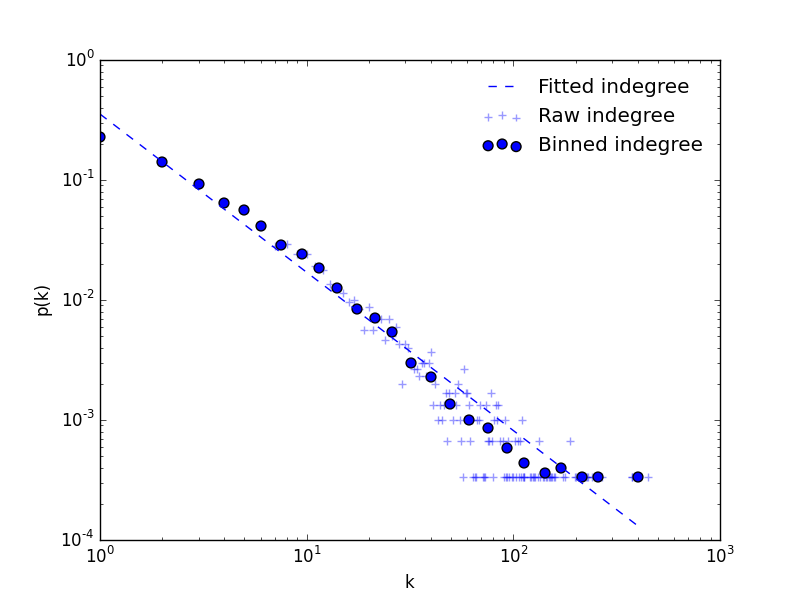
\includegraphics[width=0.75\linewidth]{figs/indegree.png}
\end{figure}
\small{The probability density function (PDF) of indegrees, excluding the nodes with zero degrees. The power-law fitting parameters $\alpha=-1.319$ and standard error (i.e., RMSE) $\sigma= 0.14$ (The power-law distributions are formulated with: $p(x)\propto x^{\alpha}$).}
\end{frame}


\begin{frame}
\frametitle{Distribution of Outdegrees}
\begin{figure}
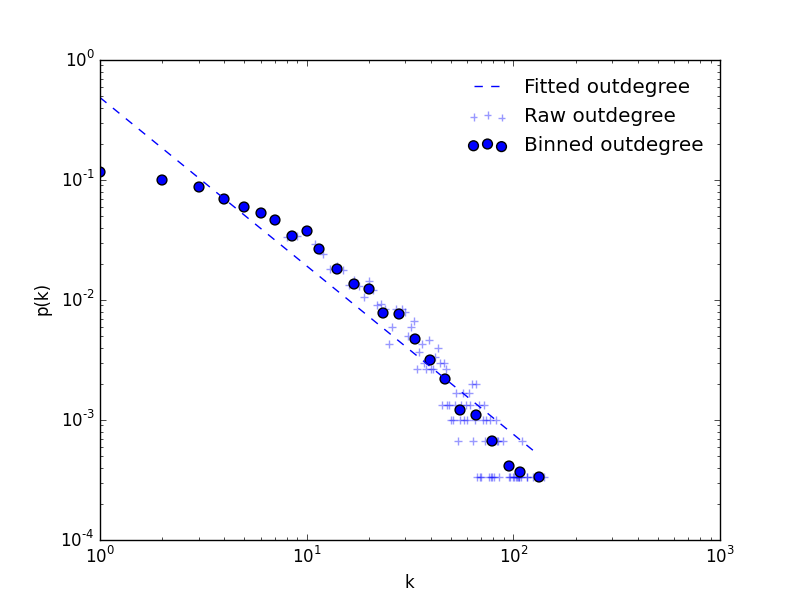
\includegraphics[width=0.8\linewidth]{figs/outdegree.png}
\end{figure}
\small{The probability density function (PDF) of outdegrees, excluding the nodes with zero degrees. The power-law fitting parameters $\alpha=-1.403$ and standard error (i.e., RMSE) $\sigma= 0.21$.}
\end{frame}

\begin{frame}
\frametitle{Distribution of Outdegrees (Splitting)}
\begin{figure}
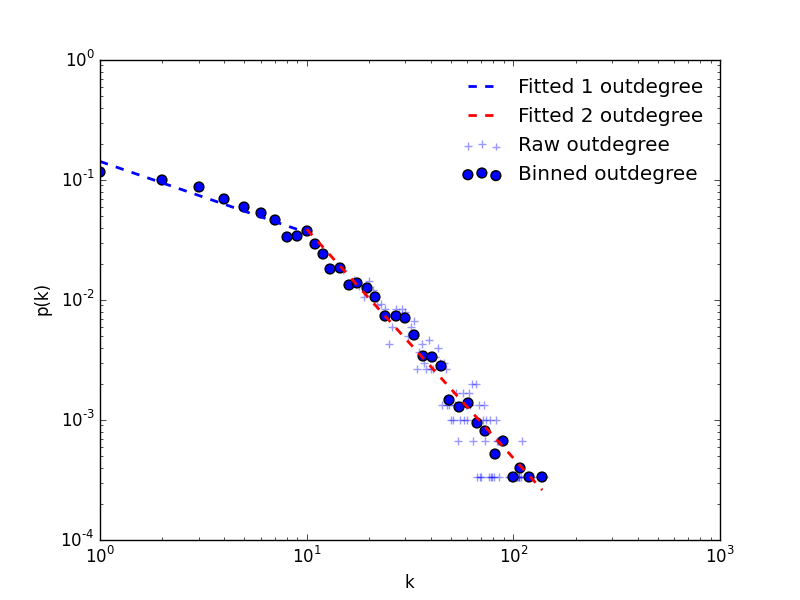
\includegraphics[width=0.75\linewidth]{figs/outdegree_split.png}
\end{figure}
\small{Splitting outdegree at $k=10$, the power-law fitting parameters in the first range $\alpha=-0.593$ and standard error (i.e., RMSE) $\sigma= 0.05$; $\alpha=-1.908$ and $\sigma= 0.08$ in the second range.}
\end{frame}

\begin{frame}
\frametitle{Distribution of Instrength}
\begin{figure}
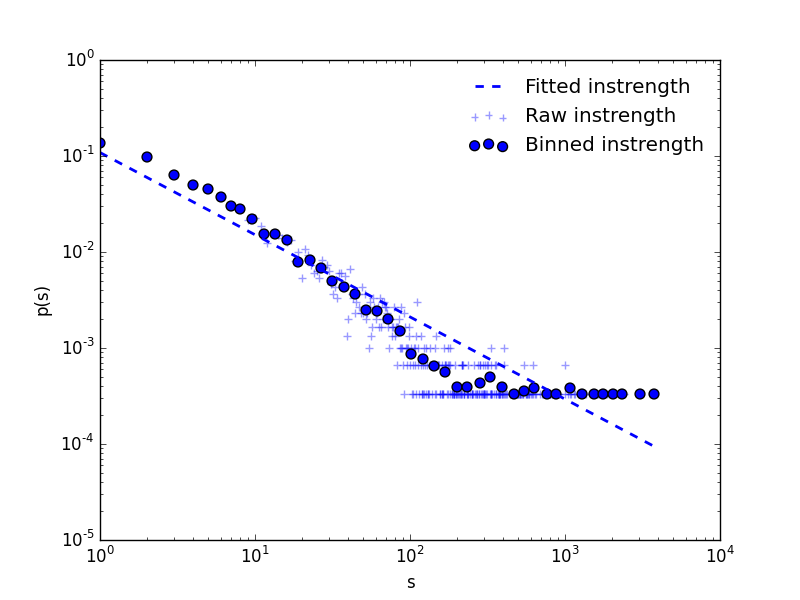
\includegraphics[width=0.8\linewidth]{figs/instrength.png}
\end{figure}
\small{The power-law fitting parameters $\alpha=-0.8562$ and standard error (i.e., RMSE) $\sigma= 0.24$.}
\end{frame}

\begin{frame}
\frametitle{Distribution of Instrength}
\begin{figure}
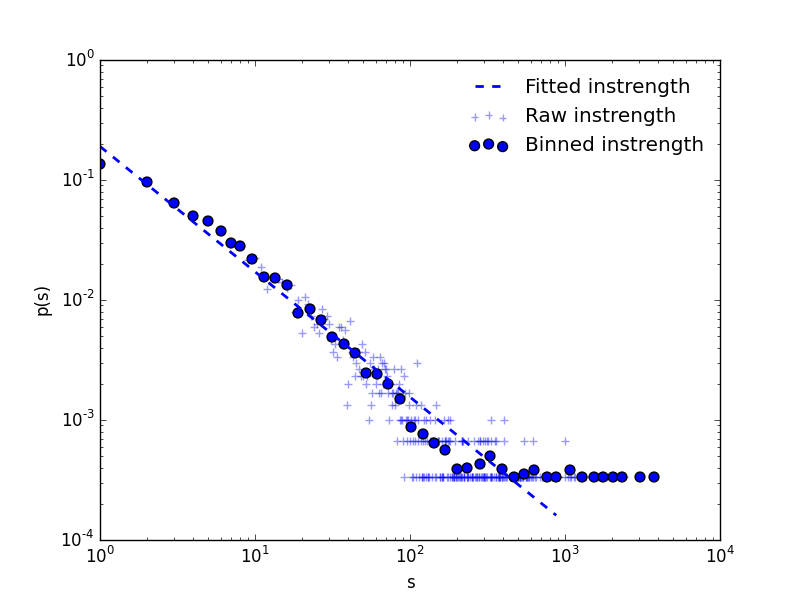
\includegraphics[width=0.8\linewidth]{figs/instrength_1000.png}
\end{figure}
\small{If excluding the nodes with instrength larger than $1000$, the power-law fitting parameters $\alpha=-1.044$ and standard error (i.e., RMSE) $\sigma= 0.13$.}
\end{frame}


\begin{frame}
\frametitle{Distribution of Outstrength}
\begin{figure}
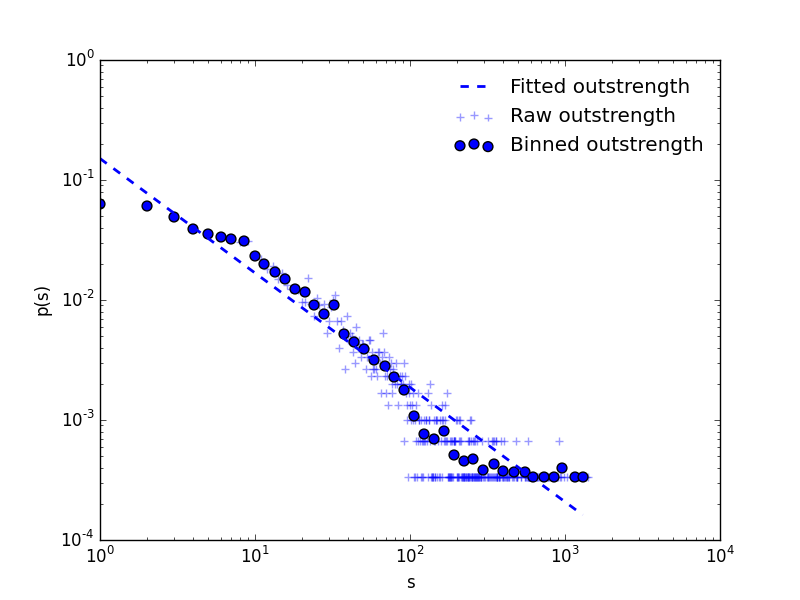
\includegraphics[width=0.8\linewidth]{figs/outstrength.png}
\end{figure}
\small{The power-law fitting parameters $\alpha=-0.9535$ and standard error (i.e., RMSE) $\sigma= 0.16$.}
\end{frame}

\begin{frame}
\frametitle{Distribution of Outstrength (Splitting)}
\begin{figure}
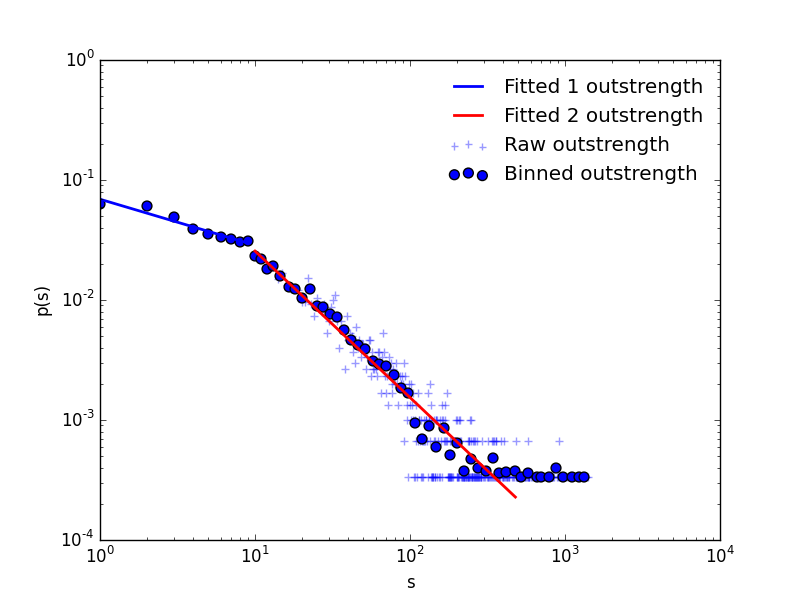
\includegraphics[width=0.8\linewidth]{figs/outstrength_split.png}
\end{figure}
\small{Fitting the nodes with outstrength in the range of $[1,500]$ and splitting outdegree at $k=10$, the power-law fitting parameters in the first range $\alpha=-0.383$ and standard error (i.e., RMSE) $\sigma= 0.03$; $\alpha=-1.22$ and $\sigma= 0.09$ in the second range.}
\end{frame}


\begin{frame}
\frametitle{Dependence of Indegrees and Outdegrees}
\begin{figure}
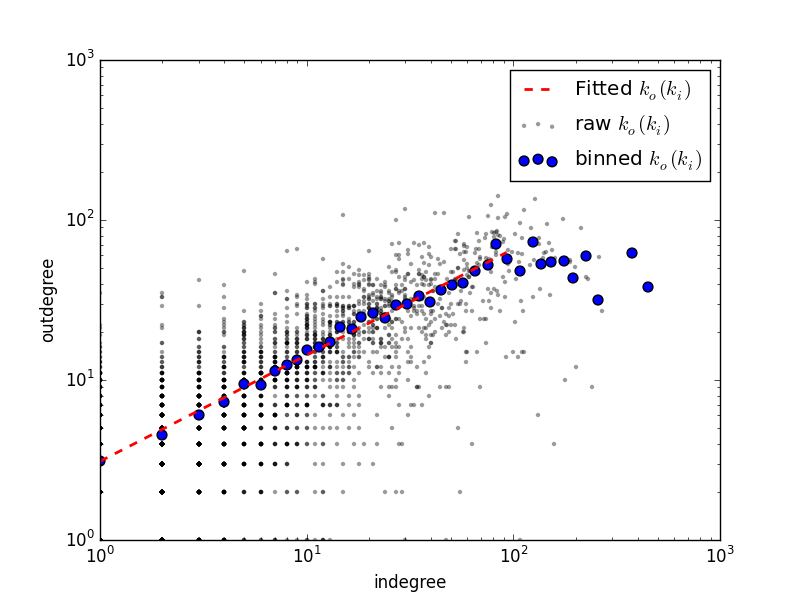
\includegraphics[width=0.8\linewidth]{figs/out_in_degree.png}
\end{figure}
\small{Fitting the nodes with indegree in the range of $[1, 100]$, the power-law fitting parameters $\alpha=0.6638$ and standard error (i.e., RMSE) $\sigma= 0.03$.}
\end{frame}

\begin{frame}
\frametitle{Dependence of Outdegrees and Indegrees}
\begin{figure}
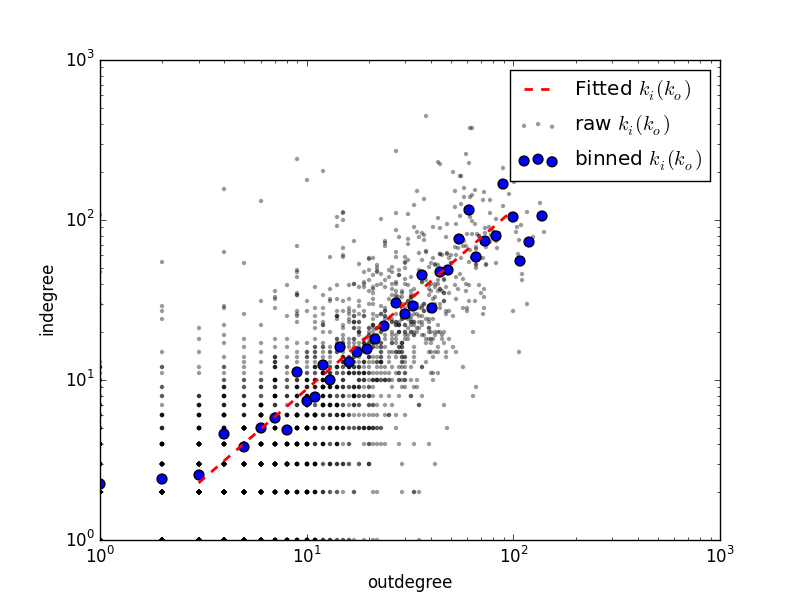
\includegraphics[width=0.8\linewidth]{figs/in_out_degree.png}
\end{figure}
\small{Fitting the nodes with outdegree in the range of $[3, 100]$, the power-law fitting parameters $\alpha=1.121 $ and standard error (i.e., RMSE) $\sigma= 0.09$.}
\end{frame}


\begin{frame}
\frametitle{Dependence of Instrength and Outstrength}
\begin{figure}
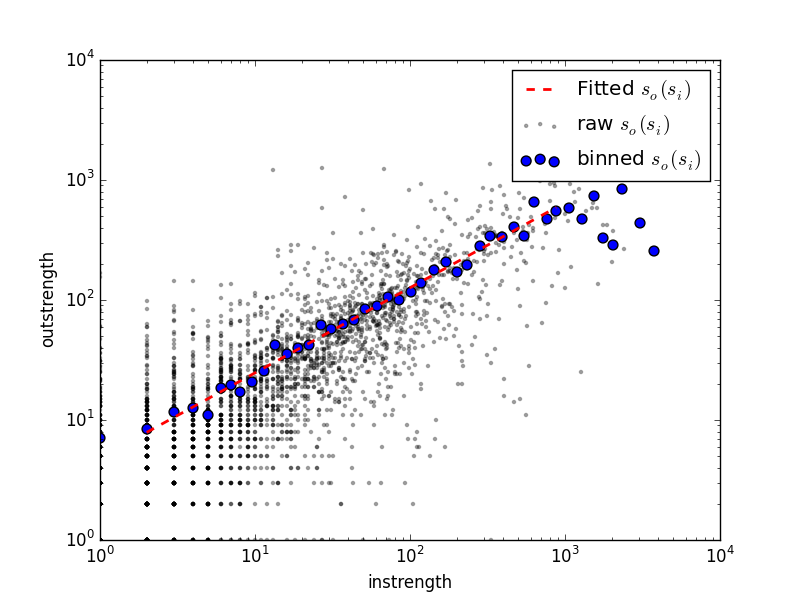
\includegraphics[width=0.8\linewidth]{figs/out_in_strength.png}
\end{figure}
\small{Fitting the nodes with instrength in the range of $[2, 1000]$, the power-law fitting parameters $\alpha=0.7094$ and standard error (i.e., RMSE) $\sigma= 0.06$.}
\end{frame}


\begin{frame}
\frametitle{Dependence of Outstrength and Instrength}
\begin{figure}
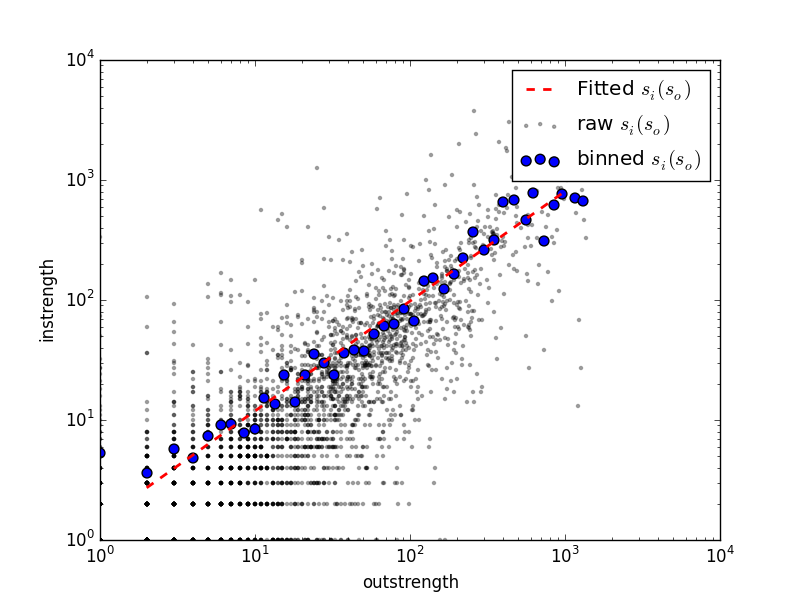
\includegraphics[width=0.8\linewidth]{figs/in_out_strength.png}
\end{figure}
\small{Fitting the nodes with instrength in the range of $[2, 1000]$, the power-law fitting parameters $\alpha=0.9154$ and standard error (i.e., RMSE) $\sigma= 0.12$.}
\end{frame}


\begin{frame}
\frametitle{Dependence of Indegree and Avg. Indegree of Predecessors}
\begin{figure}
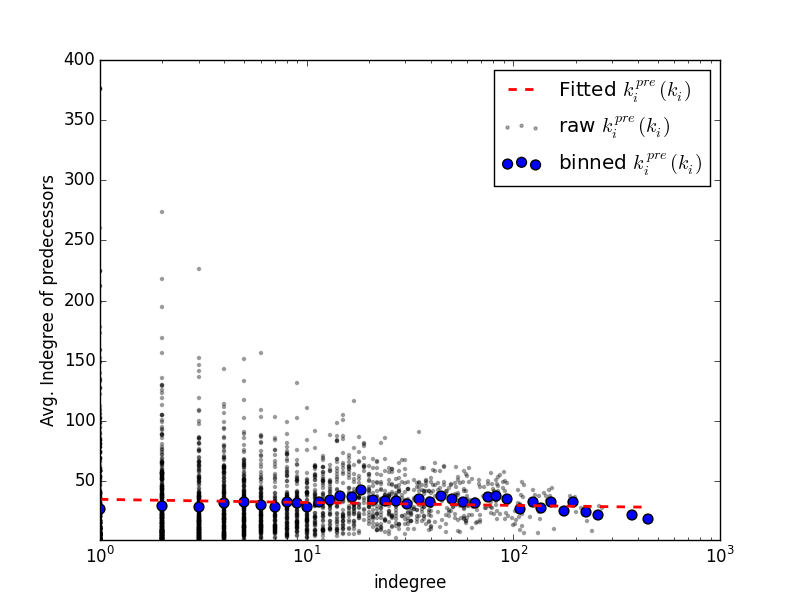
\includegraphics[width=0.8\linewidth]{figs/pre_in_in_d.png}
\end{figure}
\small{The power-law fitting parameters $\alpha=-0.03401$ and standard error (i.e., RMSE) $\sigma= 0.07$.}
\end{frame}

\begin{frame}
\frametitle{Dependence of Indegree and Avg. Outdegree of Predecessors}
\begin{figure}
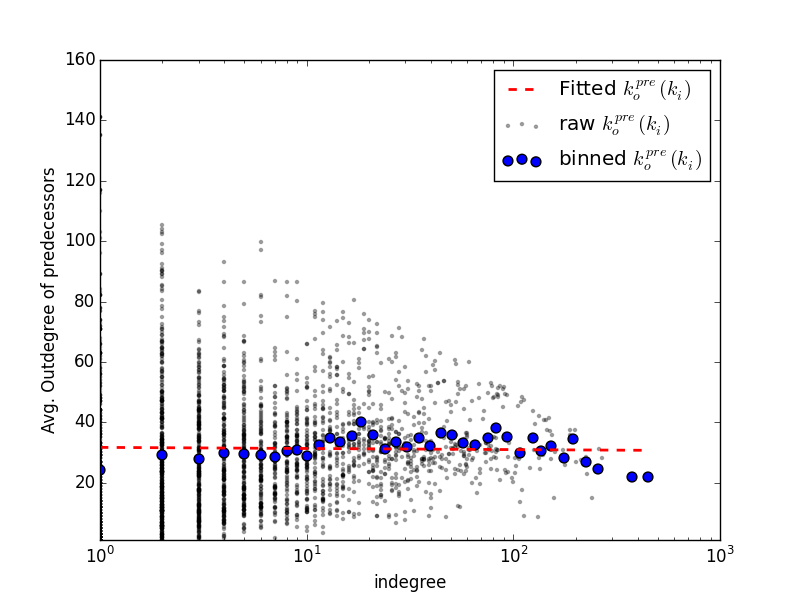
\includegraphics[width=0.8\linewidth]{figs/pre_out_in_d.png}
\end{figure}
\small{The power-law fitting parameters $\alpha=-0.005108$ and standard error (i.e., RMSE) $\sigma= 0.05$.}
\end{frame}

\begin{frame}
\frametitle{Dependence of Indegree and Avg. Indegree of Successors}
\begin{figure}
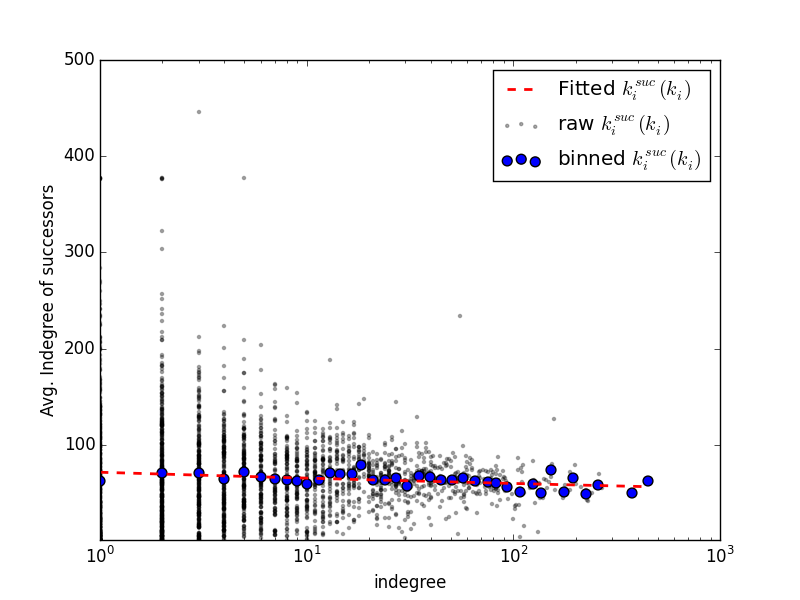
\includegraphics[width=0.8\linewidth]{figs/suc_in_in_d.png}
\end{figure}
\small{The power-law fitting parameters $\alpha=-0.03862$ and standard error (i.e., RMSE) $\sigma= 0.04$.}
\end{frame}

\begin{frame}
\frametitle{Dependence of Indegree and Avg. Outdegree of Successors}
\begin{figure}
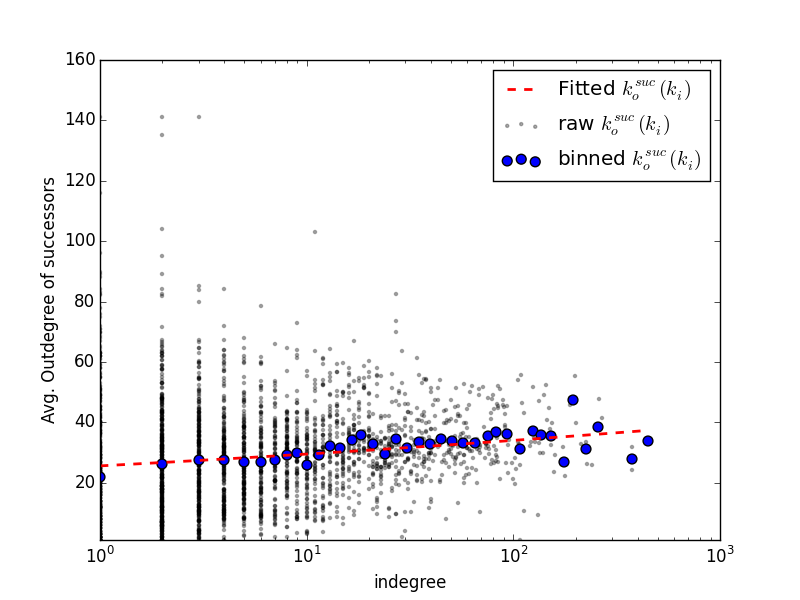
\includegraphics[width=0.8\linewidth]{figs/suc_out_in_d.png}
\end{figure}
\small{The power-law fitting parameters $\alpha=0.06204$ and standard error (i.e., RMSE) $\sigma= 0.04$.}
\end{frame}

\begin{frame}
\frametitle{Dependence of Outdegree and Avg. Indegree of Predecessors}
\begin{figure}
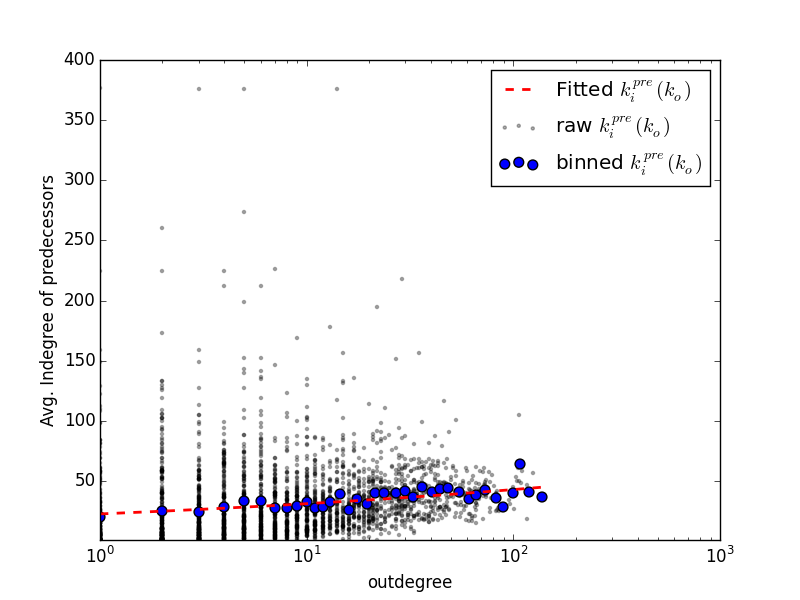
\includegraphics[width=0.8\linewidth]{figs/pre_in_out_d.png}
\end{figure}
\small{The power-law fitting parameters $\alpha=0.1387$ and standard error (i.e., RMSE) $\sigma= 0.06$.}
\end{frame}

\begin{frame}
\frametitle{Dependence of Outdegree and Avg. Outdegree of Predecessors}
\begin{figure}
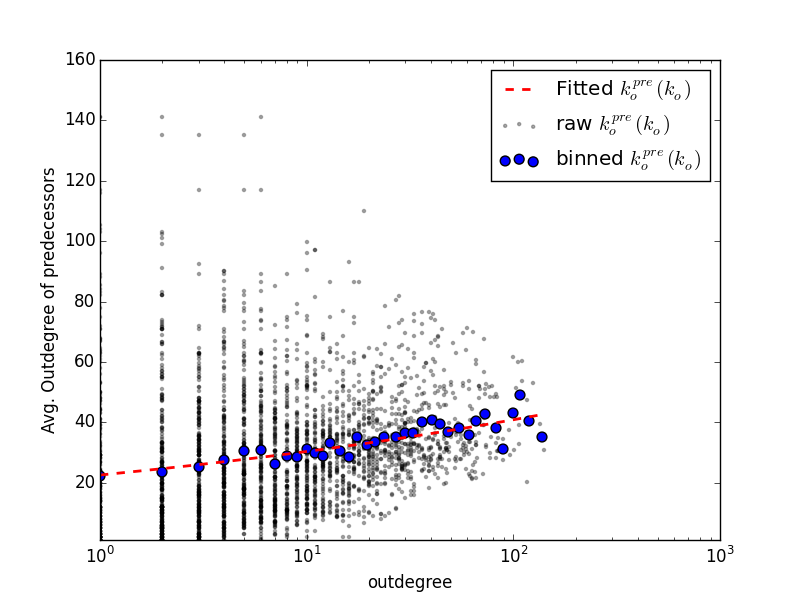
\includegraphics[width=0.8\linewidth]{figs/pre_out_out_d.png}
\end{figure}
\small{The power-law fitting parameters $\alpha=0.1293$ and standard error (i.e., RMSE) $\sigma= 0.03$.}
\end{frame}

\begin{frame}
\frametitle{Dependence of Outdegree and Avg. Indegree of Successors}
\begin{figure}
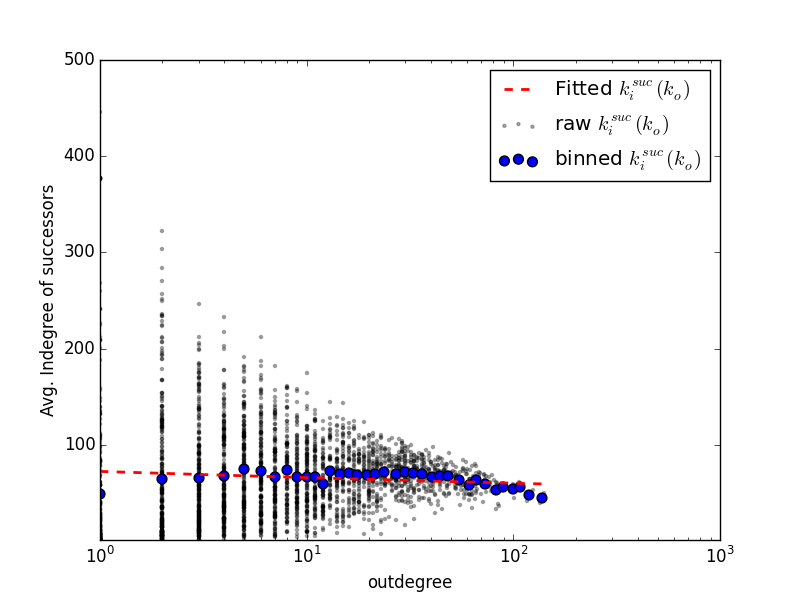
\includegraphics[width=0.8\linewidth]{figs/suc_in_out_d.png}
\end{figure}
\small{The power-law fitting parameters $\alpha=-0.04032$ and standard error (i.e., RMSE) $\sigma=0.05$.}
\end{frame}


\begin{frame}
\frametitle{Dependence of Outdegree and Avg. Outdegree of Successors}
\begin{figure}
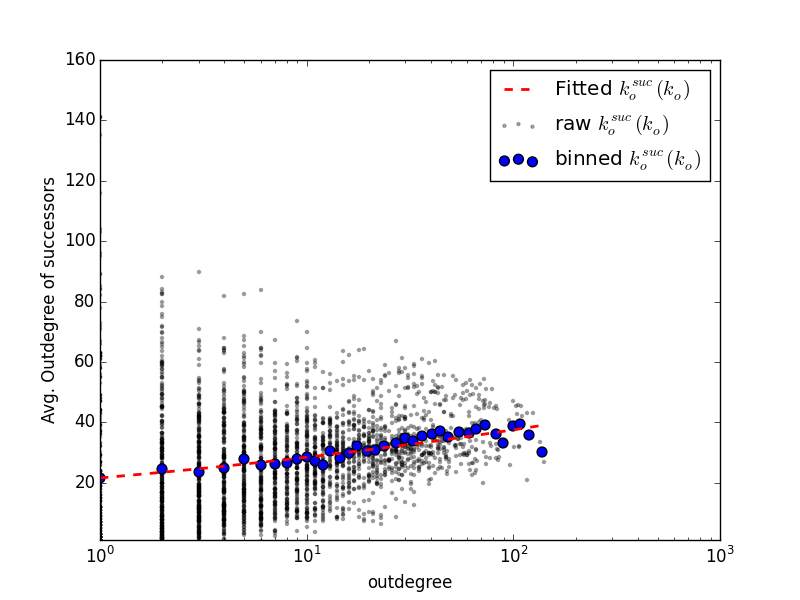
\includegraphics[width=0.8\linewidth]{figs/suc_out_out_d.png}
\end{figure}
\small{The power-law fitting parameters $\alpha=0.1202$ and standard error (i.e., RMSE) $\sigma=0.02$.}
\end{frame}


\begin{frame}
\frametitle{Dependence of Instrength and Avg. Instrength of Predecessors}
\begin{figure}
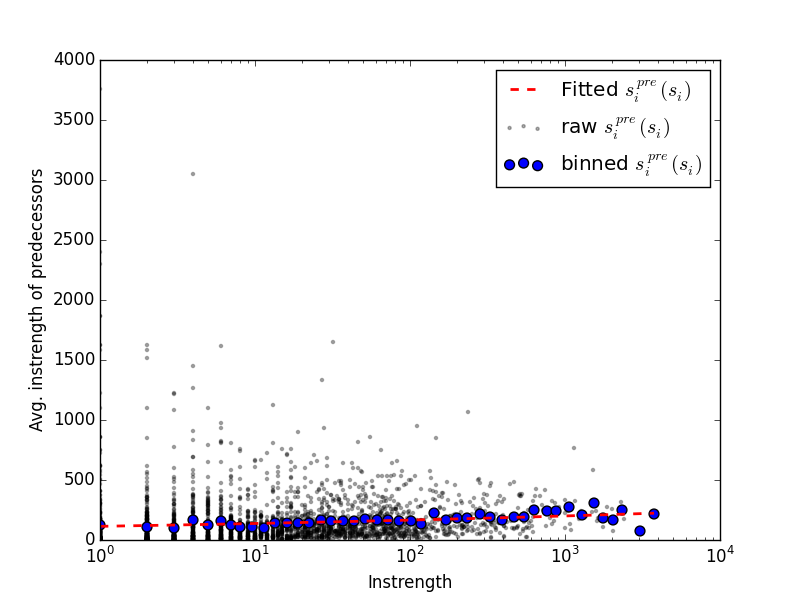
\includegraphics[width=0.8\linewidth]{figs/pre_in_in_s.png}
\end{figure}
\small{The power-law fitting parameters $\alpha=0.08118$ and standard error (i.e., RMSE) $\sigma=0.09$.}
\end{frame}

\begin{frame}
\frametitle{Dependence of Instrength and Avg. Outstrength of Predecessors}
\begin{figure}
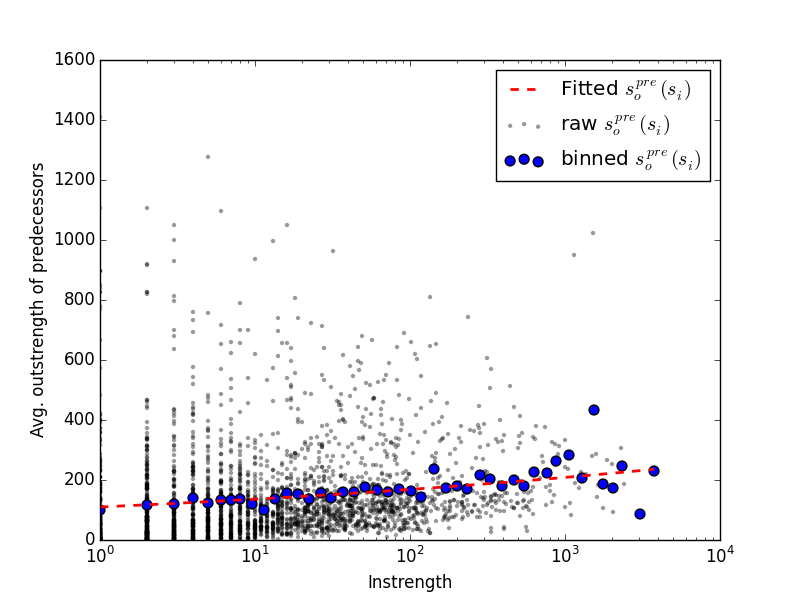
\includegraphics[width=0.8\linewidth]{figs/pre_out_in_s.png}
\end{figure}
\small{The power-law fitting parameters $\alpha=0.09193$ and standard error (i.e., RMSE) $\sigma=0.09$.}
\end{frame}


\begin{frame}
\frametitle{Dependence of Instrength and Avg. Instrength of Successors}
\begin{figure}
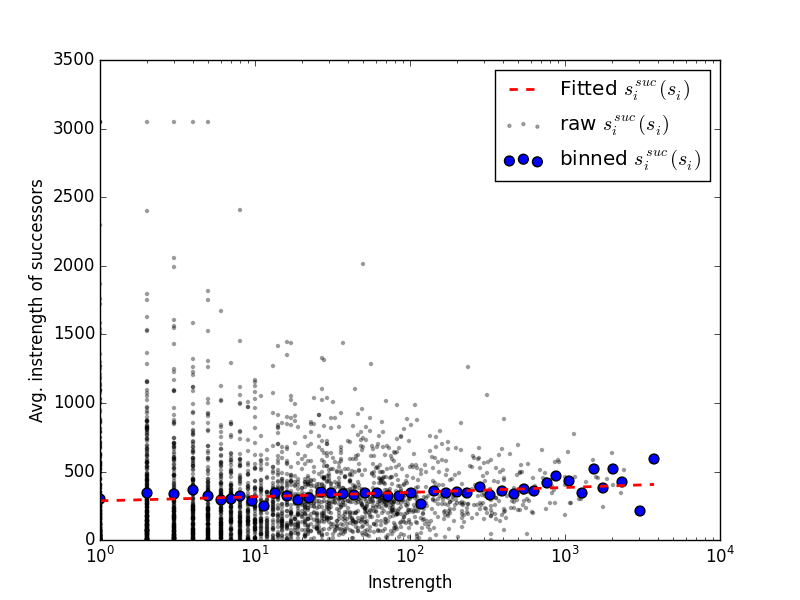
\includegraphics[width=0.8\linewidth]{figs/suc_in_in_s.png}
\end{figure}
\small{The power-law fitting parameters $\alpha=0.04223$ and standard error (i.e., RMSE) $\sigma=0.06$.}
\end{frame}


\begin{frame}
\frametitle{Dependence of Instrength and Avg. Outstrength of Successors}
\begin{figure}
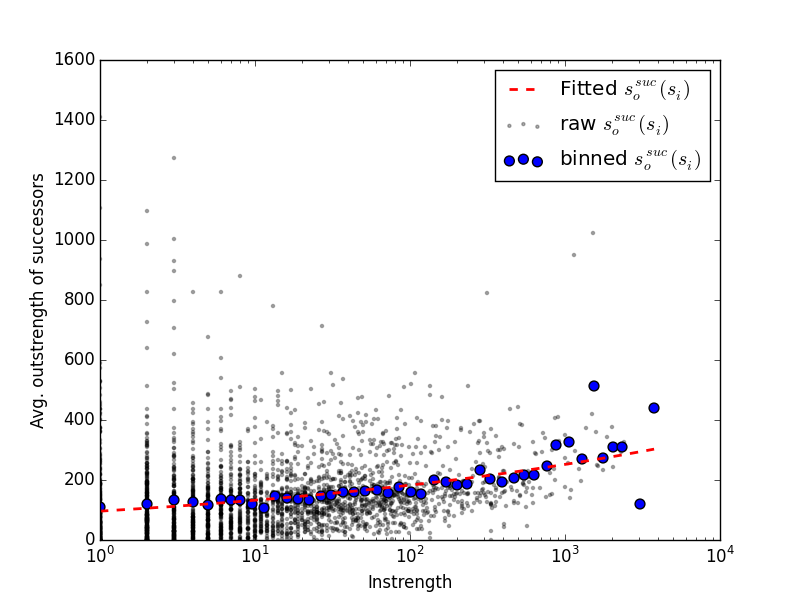
\includegraphics[width=0.8\linewidth]{figs/suc_out_in_s.png}
\end{figure}
\small{The power-law fitting parameters $\alpha=0.1385$ and standard error (i.e., RMSE) $\sigma=0.08$.}
\end{frame}

\begin{frame}
\frametitle{Dependence of Outstrength and Avg. Instrength of Predecessors}
\begin{figure}
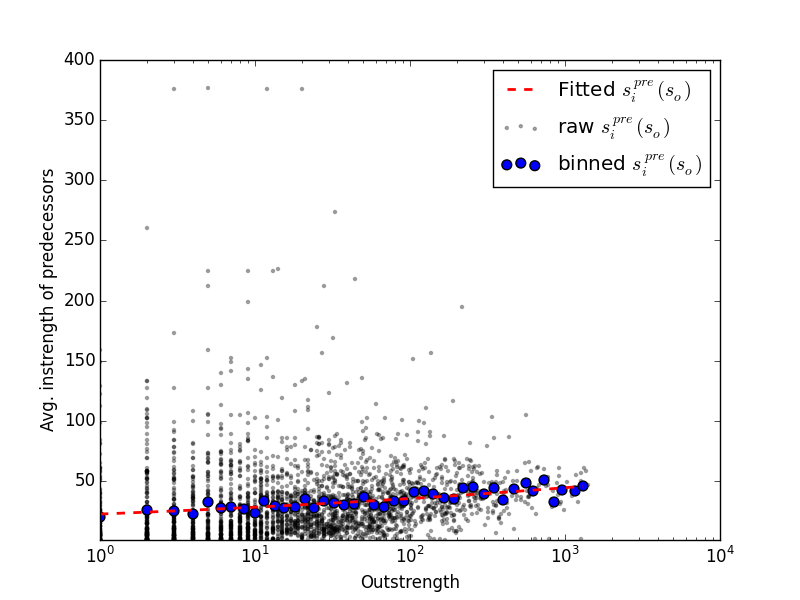
\includegraphics[width=0.8\linewidth]{figs/pre_in_out_s.png}
\end{figure}
\small{The power-law fitting parameters $\alpha=0.09821$ and standard error (i.e., RMSE) $\sigma=0.04$.}
\end{frame}

\begin{frame}
\frametitle{Dependence of Outstrength and Avg. Outstrength of Predecessors}
\begin{figure}
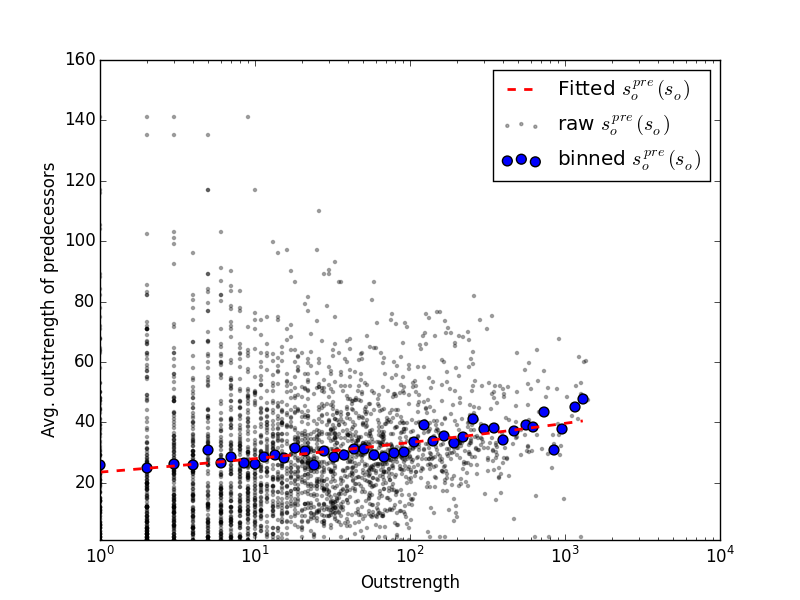
\includegraphics[width=0.8\linewidth]{figs/pre_out_out_s.png}
\end{figure}
\small{The power-law fitting parameters $\alpha=0.07583$ and standard error (i.e., RMSE) $\sigma=0.03$.}
\end{frame}

\begin{frame}
\frametitle{Dependence of Outstrength and Avg. Instrength of Successors}
\begin{figure}
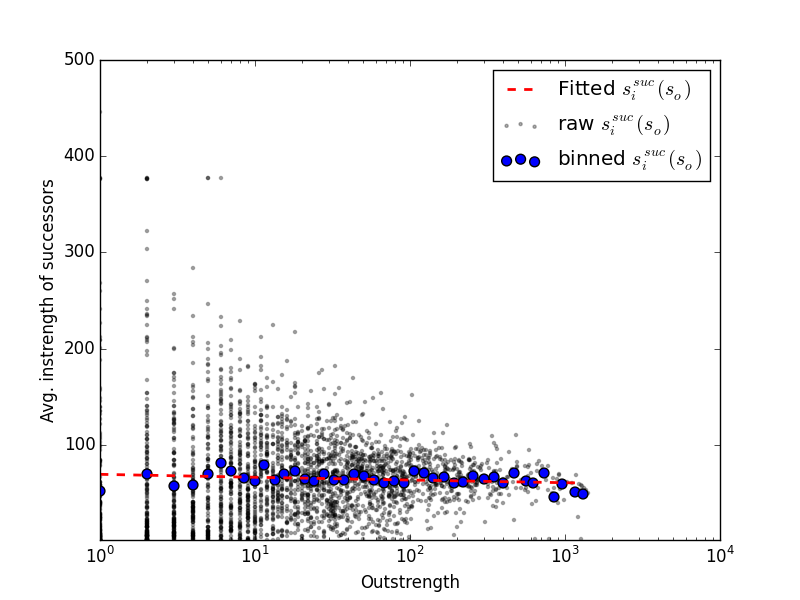
\includegraphics[width=0.8\linewidth]{figs/suc_in_out_s.png}
\end{figure}
\small{The power-law fitting parameters $\alpha=-0.01945$ and standard error (i.e., RMSE) $\sigma=0.04$.}
\end{frame}


\begin{frame}
\frametitle{Dependence of Outstrength and Avg. Outstrength of Successors}
\begin{figure}
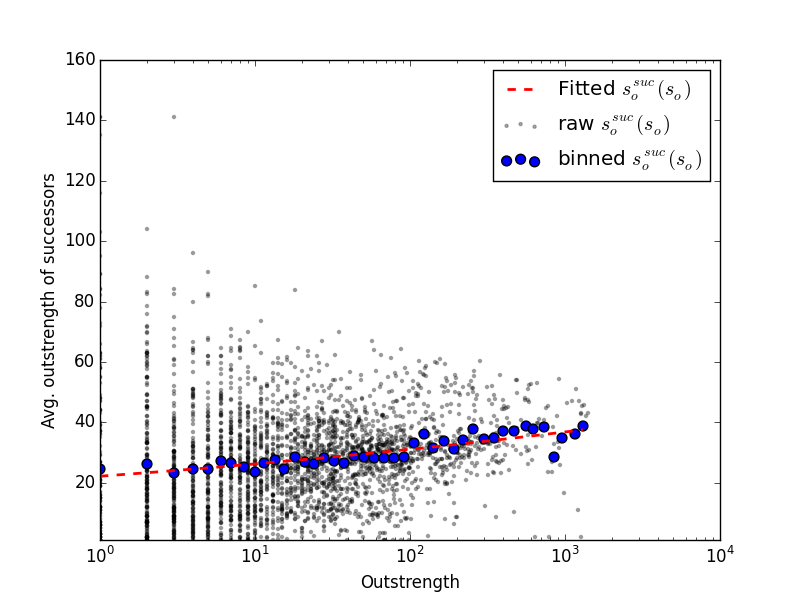
\includegraphics[width=0.8\linewidth]{figs/suc_out_out_s.png}
\end{figure}
\small{The power-law fitting parameters $\alpha=0.0736$ and standard error (i.e., RMSE) $\sigma=0.03$.}
\end{frame}

%------------------------------------------------

\begin{frame}
\Huge{\centerline{The End}}
\end{frame}

%----------------------------------------------------------------------------------------

\end{document} 